%% bare_jrnl.tex
%% V1.4b
%% 2015/08/26
%% by Michael Shell
%% see http://www.michaelshell.org/
%% for current contact information.
%%
%% This is a skeleton file demonstrating the use of IEEEtran.cls
%% (requires IEEEtran.cls version 1.8b or later) with an IEEE
%% journal paper.
%%
%% Support sites:
%% http://www.michaelshell.org/tex/ieeetran/
%% http://www.ctan.org/pkg/ieeetran
%% and
%% http://www.ieee.org/

%%*************************************************************************
%% Legal Notice:
%% This code is offered as-is without any warranty either expressed or
%% implied; without even the implied warranty of MERCHANTABILITY or
%% FITNESS FOR A PARTICULAR PURPOSE!
%% User assumes all risk.
%% In no event shall the IEEE or any contributor to this code be liable for
%% any damages or losses, including, but not limited to, incidental,
%% consequential, or any other damages, resulting from the use or misuse
%% of any information contained here.
%%
%% All comments are the opinions of their respective authors and are not
%% necessarily endorsed by the IEEE.
%%
%% This work is distributed under the LaTeX Project Public License (LPPL)
%% ( http://www.latex-project.org/ ) version 1.3, and may be freely used,
%% distributed and modified. A copy of the LPPL, version 1.3, is included
%% in the base LaTeX documentation of all distributions of LaTeX released
%% 2003/12/01 or later.
%% Retain all contribution notices and credits.
%% ** Modified files should be clearly indicated as such, including  **
%% ** renaming them and changing author support contact information. **
%%*************************************************************************


% *** Authors should verify (and, if needed, correct) their LaTeX system  ***
% *** with the testflow diagnostic prior to trusting their LaTeX platform ***
% *** with production work. The IEEE's font choices and paper sizes can   ***
% *** trigger bugs that do not appear when using other class files.       ***                          ***
% The testflow support page is at:
% http://www.michaelshell.org/tex/testflow/



\documentclass[journal]{IEEEtran}
%
% If IEEEtran.cls has not been installed into the LaTeX system files,
% manually specify the path to it like:
% \documentclass[journal]{../sty/IEEEtran}





% Some very useful LaTeX packages include:
% (uncomment the ones you want to load)


% *** MISC UTILITY PACKAGES ***
%
%\usepackage{ifpdf}
% Heiko Oberdiek's ifpdf.sty is very useful if you need conditional
% compilation based on whether the output is pdf or dvi.
% usage:
% \ifpdf
%   % pdf code
% \else
%   % dvi code
% \fi
% The latest version of ifpdf.sty can be obtained from:
% http://www.ctan.org/pkg/ifpdf
% Also, note that IEEEtran.cls V1.7 and later provides a builtin
% \ifCLASSINFOpdf conditional that works the same way.
% When switching from latex to pdflatex and vice-versa, the compiler may
% have to be run twice to clear warning/error messages.






% *** CITATION PACKAGES ***
%
%\usepackage{cite}
% cite.sty was written by Donald Arseneau
% V1.6 and later of IEEEtran pre-defines the format of the cite.sty package
% \cite{} output to follow that of the IEEE. Loading the cite package will
% result in citation numbers being automatically sorted and properly
% "compressed/ranged". e.g., [1], [9], [2], [7], [5], [6] without using
% cite.sty will become [1], [2], [5]--[7], [9] using cite.sty. cite.sty's
% \cite will automatically add leading space, if needed. Use cite.sty's
% noadjust option (cite.sty V3.8 and later) if you want to turn this off
% such as if a citation ever needs to be enclosed in parenthesis.
% cite.sty is already installed on most LaTeX systems. Be sure and use
% version 5.0 (2009-03-20) and later if using hyperref.sty.
% The latest version can be obtained at:
% http://www.ctan.org/pkg/cite
% The documentation is contained in the cite.sty file itself.






% *** GRAPHICS RELATED PACKAGES ***
%
\ifCLASSINFOpdf
\usepackage[pdftex]{graphicx}
  % declare the path(s) where your graphic files are
\graphicspath{{./Figures/}}
% \graphicspath{{../pdf/}{../jpeg/}}
  % and their extensions so you won't have to specify these with
  % every instance of \includegraphics
  %\DeclareGraphicsExtensions{.pdf,.jpeg,.png}
\else
  % or other class option (dvipsone, dvipdf, if not using dvips). graphicx
  % will default to the driver specified in the system graphics.cfg if no
  % driver is specified.
  % \usepackage[dvips]{graphicx}
  % declare the path(s) where your graphic files are
  % \graphicspath{{../eps/}}
  % and their extensions so you won't have to specify these with
  % every instance of \includegraphics
  % \DeclareGraphicsExtensions{.eps}
\fi
% graphicx was written by David Carlisle and Sebastian Rahtz. It is
% required if you want graphics, photos, etc. graphicx.sty is already
% installed on most LaTeX systems. The latest version and documentation
% can be obtained at:
% http://www.ctan.org/pkg/graphicx
% Another good source of documentation is "Using Imported Graphics in
% LaTeX2e" by Keith Reckdahl which can be found at:
% http://www.ctan.org/pkg/epslatex
%
% latex, and pdflatex in dvi mode, support graphics in encapsulated
% postscript (.eps) format. pdflatex in pdf mode supports graphics
% in .pdf, .jpeg, .png and .mps (metapost) formats. Users should ensure
% that all non-photo figures use a vector format (.eps, .pdf, .mps) and
% not a bitmapped formats (.jpeg, .png). The IEEE frowns on bitmapped formats
% which can result in "jaggedy"/blurry rendering of lines and letters as
% well as large increases in file sizes.
%
% You can find documentation about the pdfTeX application at:
% http://www.tug.org/applications/pdftex





% *** MATH PACKAGES ***
%
%\usepackage{amsmath}
% A popular package from the American Mathematical Society that provides
% many useful and powerful commands for dealing with mathematics.
%
% Note that the amsmath package sets \interdisplaylinepenalty to 10000
% thus preventing page breaks from occurring within multiline equations. Use:
%\interdisplaylinepenalty=2500
% after loading amsmath to restore such page breaks as IEEEtran.cls normally
% does. amsmath.sty is already installed on most LaTeX systems. The latest
% version and documentation can be obtained at:
% http://www.ctan.org/pkg/amsmath





% *** SPECIALIZED LIST PACKAGES ***
%
%\usepackage{algorithmic}
% algorithmic.sty was written by Peter Williams and Rogerio Brito.
% This package provides an algorithmic environment fo describing algorithms.
% You can use the algorithmic environment in-text or within a figure
% environment to provide for a floating algorithm. Do NOT use the algorithm
% floating environment provided by algorithm.sty (by the same authors) or
% algorithm2e.sty (by Christophe Fiorio) as the IEEE does not use dedicated
% algorithm float types and packages that provide these will not provide
% correct IEEE style captions. The latest version and documentation of
% algorithmic.sty can be obtained at:
% http://www.ctan.org/pkg/algorithms
% Also of interest may be the (relatively newer and more customizable)
% algorithmicx.sty package by Szasz Janos:
% http://www.ctan.org/pkg/algorithmicx




% *** ALIGNMENT PACKAGES ***
%
\usepackage{multirow}
\usepackage{array}

% Frank Mittelbach's and David Carlisle's array.sty patches and improves
% the standard LaTeX2e array and tabular environments to provide better
% appearance and additional user controls. As the default LaTeX2e table
% generation code is lacking to the point of almost being broken with
% respect to the quality of the end results, all users are strongly
% advised to use an enhanced (at the very least that provided by array.sty)
% set of table tools. array.sty is already installed on most systems. The
% latest version and documentation can be obtained at:
% http://www.ctan.org/pkg/array


% IEEEtran contains the IEEEeqnarray family of commands that can be used to
% generate multiline equations as well as matrices, tables, etc., of high
% quality.




% *** SUBFIGURE PACKAGES ***
%\ifCLASSOPTIONcompsoc
%  \usepackage[caption=false,font=normalsize,labelfont=sf,textfont=sf]{subfig}
%\else
%  \usepackage[caption=false,font=footnotesize]{subfig}
%\fi
% subfig.sty, written by Steven Douglas Cochran, is the modern replacement
% for subfigure.sty, the latter of which is no longer maintained and is
% incompatible with some LaTeX packages including fixltx2e. However,
% subfig.sty requires and automatically loads Axel Sommerfeldt's caption.sty
% which will override IEEEtran.cls' handling of captions and this will result
% in non-IEEE style figure/table captions. To prevent this problem, be sure
% and invoke subfig.sty's "caption=false" package option (available since
% subfig.sty version 1.3, 2005/06/28) as this is will preserve IEEEtran.cls
% handling of captions.
% Note that the Computer Society format requires a larger sans serif font
% than the serif footnote size font used in traditional IEEE formatting
% and thus the need to invoke different subfig.sty package options depending
% on whether compsoc mode has been enabled.
%
% The latest version and documentation of subfig.sty can be obtained at:
% http://www.ctan.org/pkg/subfig




% *** FLOAT PACKAGES ***
%
%\usepackage{fixltx2e}
% fixltx2e, the successor to the earlier fix2col.sty, was written by
% Frank Mittelbach and David Carlisle. This package corrects a few problems
% in the LaTeX2e kernel, the most notable of which is that in current
% LaTeX2e releases, the ordering of single and double column floats is not
% guaranteed to be preserved. Thus, an unpatched LaTeX2e can allow a
% single column figure to be placed prior to an earlier double column
% figure.
% Be aware that LaTeX2e kernels dated 2015 and later have fixltx2e.sty's
% corrections already built into the system in which case a warning will
% be issued if an attempt is made to load fixltx2e.sty as it is no longer
% needed.
% The latest version and documentation can be found at:
% http://www.ctan.org/pkg/fixltx2e


%\usepackage{stfloats}
% stfloats.sty was written by Sigitas Tolusis. This package gives LaTeX2e
% the ability to do double column floats at the bottom of the page as well
% as the top. (e.g., "\begin{figure*}[!b]" is not normally possible in
% LaTeX2e). It also provides a command:
%\fnbelowfloat
% to enable the placement of footnotes below bottom floats (the standard
% LaTeX2e kernel puts them above bottom floats). This is an invasive package
% which rewrites many portions of the LaTeX2e float routines. It may not work
% with other packages that modify the LaTeX2e float routines. The latest
% version and documentation can be obtained at:
% http://www.ctan.org/pkg/stfloats
% Do not use the stfloats baselinefloat ability as the IEEE does not allow
% \baselineskip to stretch. Authors submitting work to the IEEE should note
% that the IEEE rarely uses double column equations and that authors should try
% to avoid such use. Do not be tempted to use the cuted.sty or midfloat.sty
% packages (also by Sigitas Tolusis) as the IEEE does not format its papers in
% such ways.
% Do not attempt to use stfloats with fixltx2e as they are incompatible.
% Instead, use Morten Hogholm'a dblfloatfix which combines the features
% of both fixltx2e and stfloats:
%
% \usepackage{dblfloatfix}
% The latest version can be found at:
% http://www.ctan.org/pkg/dblfloatfix




%\ifCLASSOPTIONcaptionsoff
%  \usepackage[nomarkers]{endfloat}
% \let\MYoriglatexcaption\caption
% \renewcommand{\caption}[2][\relax]{\MYoriglatexcaption[#2]{#2}}
%\fi
% endfloat.sty was written by James Darrell McCauley, Jeff Goldberg and
% Axel Sommerfeldt. This package may be useful when used in conjunction with
% IEEEtran.cls'  captionsoff option. Some IEEE journals/societies require that
% submissions have lists of figures/tables at the end of the paper and that
% figures/tables without any captions are placed on a page by themselves at
% the end of the document. If needed, the draftcls IEEEtran class option or
% \CLASSINPUTbaselinestretch interface can be used to increase the line
% spacing as well. Be sure and use the nomarkers option of endfloat to
% prevent endfloat from "marking" where the figures would have been placed
% in the text. The two hack lines of code above are a slight modification of
% that suggested by in the endfloat docs (section 8.4.1) to ensure that
% the full captions always appear in the list of figures/tables - even if
% the user used the short optional argument of \caption[]{}.
% IEEE papers do not typically make use of \caption[]'s optional argument,
% so this should not be an issue. A similar trick can be used to disable
% captions of packages such as subfig.sty that lack options to turn off
% the subcaptions:
% For subfig.sty:
% \let\MYorigsubfloat\subfloat
% \renewcommand{\subfloat}[2][\relax]{\MYorigsubfloat[]{#2}}
% However, the above trick will not work if both optional arguments of
% the \subfloat command are used. Furthermore, there needs to be a
% description of each subfigure *somewhere* and endfloat does not add
% subfigure captions to its list of figures. Thus, the best approach is to
% avoid the use of subfigure captions (many IEEE journals avoid them anyway)
% and instead reference/explain all the subfigures within the main caption.
% The latest version of endfloat.sty and its documentation can obtained at:
% http://www.ctan.org/pkg/endfloat
%
% The IEEEtran \ifCLASSOPTIONcaptionsoff conditional can also be used
% later in the document, say, to conditionally put the References on a
% page by themselves.




% *** PDF, URL AND HYPERLINK PACKAGES ***
%
%\usepackage{url}
% url.sty was written by Donald Arseneau. It provides better support for
% handling and breaking URLs. url.sty is already installed on most LaTeX
% systems. The latest version and documentation can be obtained at:
% http://www.ctan.org/pkg/url
% Basically, \url{my_url_here}.




% *** Do not adjust lengths that control margins, column widths, etc. ***
% *** Do not use packages that alter fonts (such as pslatex).         ***
% There should be no need to do such things with IEEEtran.cls V1.6 and later.
% (Unless specifically asked to do so by the journal or conference you plan
% to submit to, of course. )


% correct bad hyphenation here
\hyphenation{op-tical net-works semi-conduc-tor}


\begin{document}
%
% paper title
% Titles are generally capitalized except for words such as a, an, and, as,
% at, but, by, for, in, nor, of, on, or, the, to and up, which are usually
% not capitalized unless they are the first or last word of the title.
% Linebreaks \\ can be used within to get better formatting as desired.
% Do not put math or special symbols in the title.
\title{C Compiler for the VERSAT Reconfigurable Processor}
%
%
% author names and IEEE memberships
% note positions of commas and nonbreaking spaces ( ~ ) LaTeX will not break
% a structure at a ~ so this keeps an author's name from being broken across
% two lines.
% use \thanks{} to gain access to the first footnote area
% a separate \thanks must be used for each paragraph as LaTeX2e's \thanks
% was not built to handle multiple paragraphs
%

\author{\IEEEauthorblockN{Gon\c{c}alo~R.~Santos}\\
\IEEEauthorblockA{T\'ecnico Lisboa\\
University of Lisbon\\
Email: goncalo.c.r.santos@tecnico.ulisboa.pt}
%\ifCLASSOPTIONpeerreview
%\thanks{The authors are with the INESC-ID, University of Lisbon, Portugal, contact e-mail: jose.desousa@inesc-id.pt.}% <-this % stops a space
%\fi
%\thanks{}% <-this % stops a space
\thanks{Manuscript received October 19, 2019.}}

% note the % following the last \IEEEmembership and also \thanks -
% these prevent an unwanted space from occurring between the last author name
% and the end of the author line. i.e., if you had this:
%
% \author{....lastname \thanks{...} \thanks{...} }
%                     ^------------^------------^----Do not want these spaces!
%
% a space would be appended to the last name and could cause every name on that
% line to be shifted left slightly. This is one of those "LaTeX things". For
% instance, "\textbf{A} \textbf{B}" will typeset as "A B" not "AB". To get
% "AB" then you have to do: "\textbf{A}\textbf{B}"
% \thanks is no different in this regard, so shield the last } of each \thanks
% that ends a line with a % and do not let a space in before the next \thanks.
% Spaces after \IEEEmembership other than the last one are OK (and needed) as
% you are supposed to have spaces between the names. For what it is worth,
% this is a minor point as most people would not even notice if the said evil
% space somehow managed to creep in.



% The paper headers
%\ifCLASSOPTIONpeerreview
%\markboth{IEEE Transactions on Very Large Scale Integration (VLSI) Systems,~Vol.~X, No.~Y, Month-Year}%
%         {Lopes \MakeLowercase{\textit{et al.}}: VERSAT, a Compile-Friendly Reconfigurable Processor -- Architecture}
%\fi
% The only time the second header will appear is for the odd numbered pages
% after the title page when using the twoside option.
%
% *** Note that you probably will NOT want to include the author's ***
% *** name in the headers of peer review papers.                   ***
% You can use \ifCLASSOPTIONpeerreview for conditional compilation here if
% you desire.




% If you want to put a publisher's ID mark on the page you can do it like
% this:
%\IEEEpubid{0000--0000/00\$00.00~\copyright~2015 IEEE}
% Remember, if you use this you must call \IEEEpubidadjcol in the second
% column for its text to clear the IEEEpubid mark.



% use for special paper notices
%\IEEEspecialpapernotice{(Invited Paper)}




% make the title area
\maketitle

% As a general rule, do not put math, special symbols or citations
% in the abstract or keywords.
\begin{abstract}
This paper describes de development of a {\bf C} language compiler
for {\it picoVersat}.
{\it picoVersat} is the hardware controller for {\it Versat},
coarse grain reconfigurable array.
The compiler is developed as a {\it back-end} for the {\bf lcc} retargetable
compiler.
The {\it back-end} uses a code selection tool for most operations, while some
where manually coded.
Assembly inline support was added to the {\it front-end} since it was missing
from {\bf lcc}.
The compiler was integrated into a compilation framework and extensive
testing was performed.
Finally, some limitations were highlighted, relating to the compiler and
{\it picoVersat} usage, and some efficiency considerations were addressed.

\end{abstract}

% Note that keywords are not normally used for peerreview papers.
\begin{IEEEkeywords}
Versat, CGRA, picoVersat, C-compiler, lcc {\it back-end}.
\end{IEEEkeywords}


% For peer review papers, you can put extra information on the cover
% page as needed:
% \ifCLASSOPTIONpeerreview
% \begin{center} \bfseries EDICS Category: 3-BBND \end{center}
% \fi
%
% For peerreview papers, this IEEEtran command inserts a page break and
% creates the second title. It will be ignored for other modes.
\IEEEpeerreviewmaketitle



\section{Introduction}
% The very first letter is a 2 line initial drop letter followed
% by the rest of the first word in caps.
%
% form to use if the first word consists of a single letter:
% \IEEEPARstart{A}{demo} file is ....
%
% form to use if you need the single drop letter followed by
% normal text (unknown if ever used by the IEEE):
% \IEEEPARstart{A}{}demo file is ....
%
% Some journals put the first two words in caps:
% \IEEEPARstart{T}{his demo} file is ....
%
% Here we have the typical use of a "T" for an initial drop letter
% and "HIS" in caps to complete the first word.

% You must have at least 2 lines in the paragraph with the drop letter
% (should never be an issuem
\IEEEPARstart{R}{econfigurable computation} has had a great focus
in the past decades.
Due to the fact that these systems can change their architecture dynamically to
be best suit to the task being executed, they can greatly accelerate the
execution of applications mainly in fields reigned by embedded systems, like
telecommunications, multimedia, etc~\cite{Carta06,Liu15,Lee18TACO}.
Many of these embedded applications need to have low power consumption and
reduced silicon area while still having a high number of computations done per second.

{\it Versat} is one of these architectures capable of changing
dynamically~\cite{Lopes16}.  This system uses a Data Engine in order to execute
code loops. {\it Versat}, like architectures of this type, is not designed to
run efficiently when the code has a great amount of different instructions but
rather when the code revolves around loops and repeated instructions in general.
To do the more eclectic code there is a controller that also manages {\it
Versat}, making it run and taking care of the reconfigurations.

The purpose of this work is to improve the {\it Versat} compiler solving the
issues it still has. For this, some different options will be discussed, keeping
in mind that this is not a traditional CPU architecture. This means that there
is need to study compilers in general as well as the architecture in question.

\subsection{Motivation}
\label{section:motiva}

High-level languages, like {\bf C}/{\bf C++} or Java, allow for program
development without the knowledge of the inner workings of a given
processor. Futhermore, the development is faster and programs are easier to
debug or test than using an assembly language for a specific processor. {\it
  Versat} is programmable in assembly using the {\it picoVersat} instruction
set. The assembler program available for program development is a cumbersome
form to port existing algorithms to the {\it Versat} platform, most of them
written in {\bf C} or {\bf C++}.  A compiler is essential for the test and
assessement of the {\it Versat} platform capabilities.  A first prototype
compiler, developed by Rui Santiago~\cite{Santiago2016}, exists and was used for
the development of some examples.  However, the compiler is not only not very
practical still, but also quite primitive.  It supports a limited subset of the
{\bf C} language with {\bf C++} alike method invocation, with no variables,
functions or strucutures. All programming uses the {\it picoVersat} register
names to hold values.  Furthermore, the only {\bf C++} syntax used is the method
invocation from object ({\it object.method}), but this being the only difference from
{\bf C} and since there is not the option to create multiple instances of these
objects (they act as variables), this syntax could simply be replaced with a
{\bf C} compatible syntax. This would allow for the use of a simpler compiler,
since in reality none of the extra functionalities of {\bf C++} in relation
to {\bf C} are even supposed to be used in this architecture.

\subsection{Objectives}
\label{section:objectivo}

The objective of this work is to implement the following improvements to the
Versat compiler:
\begin{itemize}
\item Partial reconfiguration: prepare the next Versat configuration by changing
  only the configuration fields that differ. Currently all configuration bits
  are updated during reconfiguration, which costs time.
\item Support a variable number of functional units: the current implementation
  assumes a fixed number of functional units, and if the hardware is changed then
  the compiler needs to change too. This improvement will lift this restriction.
\item Support variable declarations: currently all variables and objects are
  predefined and user defined variables are not supported. This improvement
  will greatly improve programmability.
\item Support function calls: currently all the code must be written in a single
  {\tt main()} function and no other functions can be called from this one. This
  improvement will allow not only for better programming practices, but also to
  make the code more extensible and easy to understand.
%\item Support constants definition:
\end{itemize}

\subsection{Challenges}
\label{section:desafio}

Building a full {\bf C} compiler on such a bare/simple instruction set requires
that most instructions need to be decomposed.  All {\bf C} language operations
that are not directly supported by the architecture have to be mapped into the
few existing ones.

Having such reduced register support in {\it picoVersat} requires the constant
memory access, and not having a {\it stack pointer}, or a {\it frame pointer},
makes function calls (in particular recursion) very impractical.

Detecting, along with regular {\bf C} code, the portions that are meant to be
computed into instructions for {\it Versat} instead of {\it picoVersat} is
difficult not only because is there a need to identify these "packs" of
instructions as well as to analyze and to compute these instructions in a
different way.

\subsection{Document structure}
\label{section:parts}

This document is divided into six sections.  The next section introduces the
{\it Versat} architecture in its present form. Section III surveys
existing {\bf C} compiler frameworks that can be adapted into a full
{\it Versat} compiler.  Section IV, Architecture, provides a first approach
into the general architecture of the compiler for the {\it Versat} platform.
The next section, Compiler development, highlights the {\it Versat} compiler
{\it back-end} internals. Section VI, Results, exposes the resulting compiler
capabilities and limitations.
Finally, some conclusions from the developed work are drawn.

\section{Versat}
\label{section:versat}

{\it Versat} is a hardware accelerator based on a reconfigurable architecture
where each peace of the program being executed can use a different composition
of functional units~\cite{deSousa12}.  It is used as a hardware accelerator for
embedded systems.  It uses a controller to generate and update the
reconfiguration.  The controller is programmable and executes programs written
in {\bf C} and assembly (specific to the architecture).  Contrary to most {\sc
  CGRA}s, which can only be fully reconfigured , {\it Versat} allows for partial
reconfiguration (where only the different configuration bits are changed), and
optimizing configuration changes.  Moreover, in this approach the configurations
are self-generated. Consequently, the host does not have to manage the
reconfiguration process, and is free to perform more useful
tasks~\cite{Lopes2017}.  {\it Versat} uses an address generation scheme that is
able to support groups expressed in a single {\sc CGRA} configuration.  Due to
the better silicon area utilization and power efficiency of heterogeneous {\sc
  CGRA}s architectures, when comparing to homogeneous ones, an heterogeneous
structure was adopted.

\subsection{picoVersat controller} % 5
\label{section:picoversat}

{\it picoVersat} is a minimal hardware controller with a reduced instruction set
and few registers, with the purpose of doing simple calculations and giving
instructions to its connected systems. Therefor, this controller is not designed
for high performance computation, even if it is able to effectively implement
simple algorithms.  It is a programmable solution which mitigates the risk of
hardware design mistakes, and helps the design and implementation of more
complex control structures.  This controller is simple and has a reduced silicon
area which allows for a low power consumption.

{\it picoVersat} is composed of four main registers:
\begin{itemize}\item
Register {\bf RA} is the accumulator and is the most relevant of the registers
in the architecture.  It can be loaded with a value read from the data interface
or with an immediate value from an instruction.  It gets the value from the
result of the operations, and is used as an operand itself along with an
immediate value or an addressed value.
\item
Register {\bf RB}, the data pointer, is used to implement indirect loads/stores
to/from the accumulator.  This register is mapped in memory which means it is
accessed by reading/writing as if accessing the data interface.
\item
Register {\bf RC} is the flag register, storing three operation flags which are
the negative, overflow, and carry flags.  Much like register {\bf RB}, this
register is also memory mapped but this one is mapped to a {\it read only}
section, being only set by the {\sc ALU}.
\item
The Program Counter, {\bf PC} register, contains the next instruction to be
fetched from the Program Memory so that it can be executed.  This register
increments for every instruction, in order to fetch the next instruction except
for branch, in which the {\bf PC} register is loaded either with an immediate
present in the branch instruction, or with the value present in {\bf RB}.  These
two types of branches implement direct and indirect branches, respectively.
\end{itemize}

For increasing the frequency, by reducing the critical path, the controller
takes two clock cycles to fetch one instruction, in pipeline.  It executes every
instruction that is fetched.  In other words, it has 2 delay slots in the case
of a branch instruction.  These delay slots can be filled with a no-operation
instruction ({\sc NOP}), but the compiler/programmer can also use them to
execute useful instructions.  For instance, in the case of a for loop, the delay
slots can be used to write the iteration count to some
register~\cite{Lopes2017}.

%\subsubsection{Instruction Set}

The instruction set that is used to run {\it picoVersat} is minimal and has only
one type.  This type has 32 bits and is divided between a 4 bit {\it opcode}
and a 28 bit immediate constant.

The operations that the controller can perform are listed in
Table~\ref{tab:isa}.  The notation used for the logic, that represents the
operations, is written with {\bf C} syntax in mind.  It is also notable that
{\it Imm} represents an immediate constant, and that {\it M$[$Imm$]$} represents
the contents in address {\it Imm} in memory.

\begin{table}[!htbp]
  \centering
  \caption{Instruction Set.}
    \begin{tabular}{|c|c|l|}
    \hline
    {\bf Mnemonic} & {\bf Opcode} & {\bf Description} \\
    \hline \hline
\multicolumn{3}{|c|}{{\bf Arithmetic / Logic}}\\
\hline \hline
    addi  & 0x0 & RA = RA + Imm; PC++\\
    \hline
    add   & 0x1 & RA = RA + M[Imm]; PC++\\
    \hline
    sub   & 0x2 & RA = RA - M[Imm]; PC++\\
    \hline
    shft  & 0x3 & RA = (Imm {\tiny $<$} 0) ? RA {\tiny $<<$} 1: RA {\tiny $>>$} 1; PC++\\
    \hline
    and   & 0x4 & RA = RA \& M[Imm]; PC++\\
    \hline
    xor   & 0x5 & RA = RA $\oplus$ M[Imm]; PC++\\
    \hline
\multicolumn{3}{|c|}{{\bf Load / Store}}\\
\hline \hline
    ldi   & 0x6 & RA = Imm; PC++\\
    \hline
    ldih  & 0x7 & RA[31:16] = Imm; PC++\\
    \hline
    rdw   & 0x8 & RA = M[Imm]; PC++\\
    \hline
    wrw   & 0x9 & M[Imm] = RA; PC++\\
    \hline
    rdwb  & 0xA & RA = M[RB+Imm]; PC++\\
    \hline
    wrwb  & 0xB & M[RB+Imm] = RA; PC++\\
    \hline
\multicolumn{3}{|c|}{{\bf Branch}}\\
\hline \hline
    beqi  & 0xC & RA == 0 ? PC = Imm: PC++; RA-\,-\\
    \hline
    beq   & 0xD & RA == 0 ? PC = M[Imm]: PC++; RA-\,-\\
    \hline
    bneqi & 0xE & RA != 0 ? PC = Imm: PC++; RA-\,-\\
    \hline
    bneq  & 0xF & RA != 0 ? PC = M[Imm]: PC++; RA-\,-\\
    \hline

    \end{tabular}
  \label{tab:isa}
\end{table}

{\tt nop}: same as {\tt addi 0}. It means No OPeration or do nothing.  The
instruction following a branch instruction is always executed due to the
instruction pipeline latency (delayed branch or slot).  Pad with {\tt nop}s if
no useful instructions can be executed.

This controller has the capability to work on its own, that is, the controller
can run the functions and operations that do not depend on the {\it Versat}
accelerator itself without it being connected, which allows the execution of
simple applications that do not have tight time constrains.


\section{Compilers selection} % 7
\label{section:compilers}

The purpose of this work is to provide a compiler that should generate
{\em picoVersat} assembly, identify and configure the {\em Versat} {\sc
  CGRA} architecture.
Since using the current compiler as a starting point is not a good option,
existing compilers were be investigated, analysed and compared in order to
select a suitable candidate for {\em picoVersat} support.

A compiler is a tool that allows the programmer to write abstract high-level
instructions and produces assembly code for the processor~\cite{aho06,cooper03}.
The assembler tool can then be used to transform the assembly instructions into
binary instructions of the processor.  The compiler can also perform semantic
error detection and data flow analysis, thus improving the required development
cycle and the generated code quality.  A good compiler can produce optimized
code as good, or sometimes better, than the manually written assembly
equivalent.

In order to transform a high-level programming language into assembly code, the
compiler tool is composed of two major phases: an analysis phase, or {\it front-end},
and a synthesis phase, or {\it back-end}.
During the analysis phase the input file is read, byte by byte, and
structured into an abstract syntax tree ({\sc AST}) containing all the relevant
information for final code generation.  The synthesis phase transforms an {\sc
  AST} into machine code assembly instructions~\cite{cooper03}.  These phases
correspond to, what is called in compiler terminology, the {\it front-end} and the
{\it back-end}, respectively.

\subsection{Standard Compilers}

{\bf gcc} is a {\bf C} compiler~\cite{Stallman:2009} with thousands of
generic and architecture specific optimizations.  Very big, lots of people
change it and maintain it, making the code very volatile, since the user
must keep up to constant changes in the code.  The purpose is not code
optimization since {\it Versat} does not provide alternative instructions
for its operations, only {\it picoVersat} could benefit of {\bf gcc} features.
It provides {\tt asm} support and many other {\bf gcc} specific {\bf C}
language extensions.

{\sc LLVM} ({\em Low Level Virtual Machine}) was born as an infrastructure for
optimization and it evolved into a full compiler with many {\it front-ends}.
A new target description is provided by a declarative domain-specific language
processed by the {\bf tblgen} tool, similar to {\bf burg} grammar descriptions.
It features a stable internal instruction set implementation and documentation.
Nowadays, the code is extensive, very large and difficult to manipulate.
The interface is complex, written in {\bf C++}, but stable.
Requires a big effort for a single person for a few months.

The {\bf lcc} is a {\bf C} compiler developed after the publication of the
{\bf BURG} papers by Proebstring, Hanson and Fraser in 1992, as a
demonstration of the concept~\cite{Fraser:burg,Fraser:gen92,Proebsting:2002}.
Up to that time {\it back-end} compiler writing was an art.
The {\bf burg} concept allowed to describe the
target architectures in a single file as well as maintaining all of them in a
single executable, a retargetable compiler.  The target architecture is
selectable by a command line option.
%
Only the {\bf C} {\it front-end} is supported with a custom made analyzer.
The input program is described in an
{\sc AST} with a well documented 32 instruction set.  Optimizations are
performed in the {\sc AST}, and through common sub-expression analysis, the tree
is converted into a {\bf DAG} ({\em Directed-Acyclic Graph}), although the
original tree is still accessible.
%
A single {\bf C} {\it front-end} reduces the complexity and line count.  Simple to
introduce new {\it back-end} since it was designed to be retargetable.  A detailed and
extensive book, and well defined {\it back-end} interface, provides a good work
basis~\cite{hanson95}.  It provides no {\tt asm} directive and it's introduction
will require changes to core of the {\it front-end} code.  However, the compiler core
is composed of 260K lines of code and any changes should be accessible.

Other compilers, like {\bf tcc} ({\em Tiny C Compiler}), {\bf pcc}, and
Amsterdam Compiler Kit ({\sc ACK}) or {\bf sdcc}, are small and simple but
not as well documented.
Also, the {\it back-end} code generation must be coded without the help of a
code selection tool.

\subsection{{\sc CGRA} Compilers}

Unlike the previous general purpose {\bf C} language compilers, {\sc CGRA}
compilers directly address the problem of configuration and reconfiguration of a
{\sc CGRA} platform.
%ver compiladores que estao no mail (TRIPS, IMAGINE, REMARC, RICA, PADDI, Chimaera, Montium, GARP, PipeRench, EGRA, SmartCell, PADDI, Pleiades, DRRA, Redefine, Colt, Matrix, FPCA, CGRA Express, and HARTMP)
%"Coarse Grained Reconfigurable Architectures in the Past 25 Years: Overview and Classification"
%%%

% refs/2013HSPSdesutter.pdf : Coarse-GrainedReconfigurableArray Architectures
%In general, the performance obtained on a programmable processor for a certain application can be defined as the reciprocal of the application execution time.
Some {\sc CGRAs}, like {\sc ADRES}, Silicon Hive, and MorphoSys are fully
dynamically reconfigurable: exactly one full reconfiguration takes place for
every execution cycle~\cite{DeSutter2010}.  Other {\sc CGRAs} like the
KressArray are fully statically reconfigurable, meaning that the {\sc CGRA} is
configured before a loop is entered, and no reconfiguration takes place during
the loop at all~\cite{DeSutter2010}.  Still other architectures feature a hybrid
reconfigurability. The RaPiD architecture features partial dynamic
reconfigurability, in which part of the bits are statically reconfigurable and
another part is dynamically reconfigurable and controlled by a small
sequencer~\cite{DeSutter2010}.  Most compiler research has been done to generate
static schedules for {\sc CGRAs}~\cite{DeSutter2010}.  Not enough details are
available in the descriptions of the compiling techniques, and few techniques
have been tried on a wide range of {\sc CGRA} architectures~\cite{DeSutter2010}.
For that reason, it is very difficult to compare the efficiency, effectiveness
and user interface of the different techniques, this is, compilation time,
quality of the generated code, and how easy it is to use and to port code to the
language used, respectively~\cite{Tuhin08}.

There are frameworks that try to compile code in usual languages to {\sc CGRAs}.
Most of these frameworks have however some limitations that do not allow them to
adapt the code fully to {\sc CGRAs}' purposes.  For example, the {\sc IMPACT}
compiler framework is used in order to parse {\bf C} source code and to get the
Intermediate Representation ({\sc IR})~\cite{Mei03}.  We can then change what
the {\it back-end} does to this {\sc IR}, to get the desired result.  However,
because of the {\sc IMPACT} {\it front-end}, most algorithms can only handle
inner loops of loop nests~\cite{Mei03}.  And since changing the {\it front-end},
as well as the {\it back-end}, is the same as creating a new compiler, most of
these frameworks have problems when there is a need to really adapt the code not
made in the specific assembly language of the {\sc CGRA}, which is supposed to run the
code.


\section{Architecture}

The development of a high-level language compiler, with variable and function
support, is the main objective of this work.  In order to achieve this goal, two
approaches can be taken: the existing compiler can be extended, or a new
compiler can be developed.

The existing compiler, although it provides valuable information, adopted many
design decisions that make the required extensions very tedious and complex.
Furthermore, there is no documentation and the lone developer is no longer
available to explain any doubts that might arise, since only the source code is
accessible.  The alternative, the development of a new compiler, can be start
from scratch or use an existing compiler.

The development of a new compiler for a rather large and complex language like
{\bf C} is a daunting task, and would require human resources beyond the scope of
this thesis.  Since several retargetable {\bf C} compilers exist, where the
{\it back-end} can be reconfigured to a new processor, a selection must be carried
out.  This options also implies that the {\it front-end} remains unchanged and that
the full {\bf C} language is implicitly support.  Consequently, all existing
{\bf C} programs that, when compiled, will fit the {\it Versat} memory can be
used.  Also, the development of new software can be made without any specific
language or architecture common knowledge other than the {\bf C} programming
language.

\subsection{Compiler selection}

After analyzing the previous options it was decided that the best approach was
to take an existing compiler and add the {\it picoVersat} {\it back-end} to it, making
it a {\it Versat} {\sc CGRA} compiler.  Even using another compiler as a
starting point some code from the existing compiler that interacts with {\it
  Versat} can be adapted to fit this model.

%start by making compiler for picoVersat
The work begins with the development of a simple compiler which is able to parse
{\bf C} code, and generate the assembly necessary to run the {\bf C} program in
the controller ({\it picoVersat}).
%In the beginning, a simple compiler that is able to parse {\bf C} code, and generate the assembly necessary to run the {\bf C} program in the controller ({\it picoVersat}), is going to be made.
Since the controller can technically work on its own without the {\it Versat}
accelerator, the compiler should also be able to reflect this.  So even with a
reduced instruction set, and limited memory, simple applications have the
capability to be run in this component.

%need to make C functions operate with the picoVersat's assembly
From the compiler candidates studied in the previous section, the {\bf lcc}
compiler seems to be the most promising approach.  It offers
an instruction selection tool that can simplify the conversion process, but no
{\tt asm} directive (not a {\bf C} standard feature) is available.
The first stage of the development process is to describe all standard
{\bf C} operations and functions using {\it picoVersat's} assembly. This will
allow the code to be parsed from {\bf C} code to the language native to the
controller which will then go through the assembler to generate the machine code
needed to run the desired program.  The assembler is already working with the
instructions described in Section~\ref{section:picoversat} so only minimal
changes will need to be done to this one, in order to generate the correct
machine code.

\subsection{picoVersat back-end}

The first stage in the development process consists in constructing a {\it back-end}
that produces {\it picoVersat} assembly code for the selected compiler.  Since
we are choosing a retargetable compiler, the introduction of a new {\it back-end} is
not a complex task.  At this stage, all {\it back-end} low-level operations must be
mapped into {\it picoVersat} assembly.  The {\it picoVersat} instruction set is
composed of a small number of instructions~(see
section~\ref{section:picoversat}) when compared with general purpose processors,
like the {\sc i386} or the {\sc ARM} processors.  Therefor, the mapping of the
{\bf C} language constructs into such a small instruction set is a complex task.
Most constructs will surely need long sequences of {\it picoVersat}
instructions.  Furthermore, some of the {\it picoVersat} registers must be
permanently assigned to compiler management tasks, such as a {\tt stack-pointer}
and a {\tt frame-pointer}, while other register may require temporary allocation
for tasks such as indirect load or save operations.  On general purpose
processors, the register set includes such registers ({\tt esp} and {\tt ebp} in
{\sc i386}, for instance) and complex load and save instructions that can
combine up to 3 registers ({\tt lea} in {\sc i386}) allowing the addressing of
field in vectors of structures.

A compiler like {\bf lcc} must also be extended to support the {\tt asm}
directive, since it does not support it yet.  Please note that such instruction,
although useful for the tasks required of this compiler, is not a part of any
{\bf C} language standard.  It started as {\bf gcc} extension and has since been
adopted by other compilers. This instruction is also useful to provide direct
control over the {\it Versat} data engine.

Figure~\ref{fig:lccPico} highlights the {\bf lcc} main blocks that need to be
modified in order to obtain a workable {\bf lcc} compiler for {\it picoVersat}.


\begin{figure}[!h]
\centering 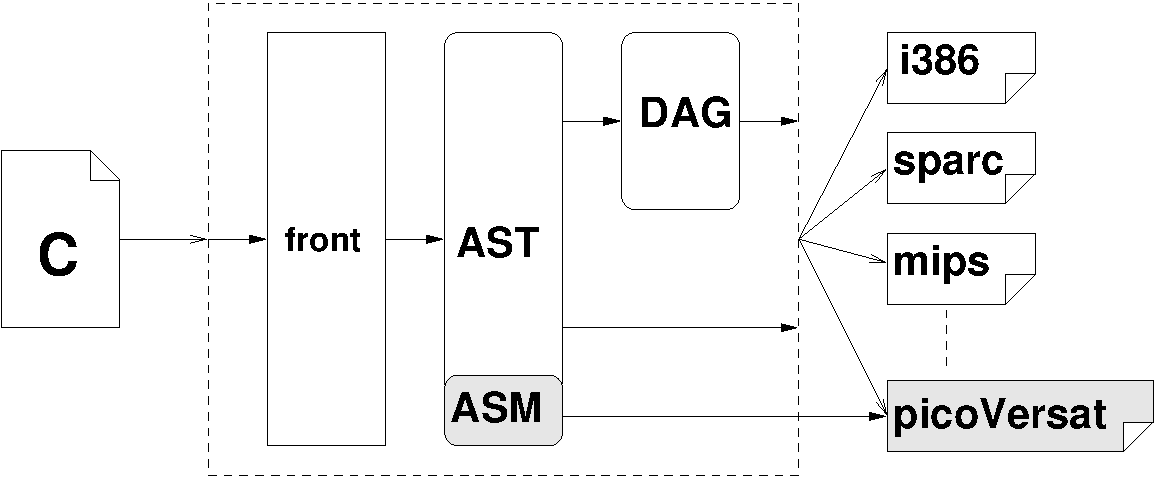
\includegraphics[width=0.80\columnwidth]{lccPico.pdf}
\caption{picoVersat {\it back-end} integration into {\bf lcc}.}
\label{fig:lccPico}
\end{figure}

\subsection{Data Engine Incorporation}

Even though {\it picoVersat} (Controller) can work on it's own for very simple
problems or auxiliary calculations, it's main purpose is to manage {\it Versat},
that is, all of its components.  In particular, the controller is meant to
manage the Data Engine in order to take full advantage of the accelerator.  This
is the biggest challenge when developing a compiler for this type of
architectures.

No matter what compiler is chosen, one thing that must hold is that all code
written needs to be compatible with the syntax used for the controller, that is,
the code used to incorporate {\it Versat} support to the compiler needs to be
compatible with the code used to compile {\it picoVersat}.  Also, in an ideal
scenario, the compiler should not need to be different for compiling code with,
or without the accelerator's functions, since the controller can operate
separately.

\section{Compiler development}
\label{chapter:develop}

The {\bf lcc} compiler is a retargetable
compiler with a single {\it front-end} for the {\bf C} programming
language ({\sc ANSI-C}).
As a retargetable compiler, multiple {\it back-ends} are available
and new ones can be easily added.
Currently, {\bf lcc} produces {\bf mips}, {\bf sparc} and
{\bf intel-x86} assembly, amongst other output formats.
Most formats, including the three referred, use an instruction
selector to generate and optimize the output assembly code.
The {\bf lcc} compiler uses a specific instruction selection
tool ({\bf lburg}), included in the compiler distribution.
Ideally, the creation of a new {\it back-end} corresponds to an
{\bf lburg} grammar description, some auxiliary functions,
and a controlling structure.

\subsection{Compiler interface}
% [asdl.pdf:6-7]
As referred, the {\it back-end} is registered in the
compiler by a single data structure,
{\tt Interface versatIR} in this case.
This structure defines the processor metrics.
In {\it Versat} all data types have a size
metric of $1$ and the align metric is also $1$,
so {\tt sizeof(char)==1} as required by the {\bf C} language.

The {\it back-end} data structure also defines some
architecture requirements.
These include the endian number format representation,
whether multiplication and division are executed
by software libraries,
whether the {\it back-end} can handle a {\bf DAG}
(directed acyclic graph), or if
it can handle passing structures to and from
functions.

The final part of the {\it back-end} data structure
defines a set of procedures to handle
specific parts of the code generation.

\subsection{Register assignment}

In order to implement the {\bf C} language constructs,
the processor must provide an accumulator to handle
return values from functions, a stack pointer to save
arguments, locals and spills, and a frame pointer to
access arguments and locals by a fixed amount.
All of these registers can be set in fixed memory positions,
but the execution degradation is significant.

The {\it picoVersat} has $16$ registers, but only registers
{\tt R1} through {\tt R12} are available as program
parameters.
The register assignment set {\tt R12} as a stack pointer, and
{\tt R11} as a frame pointer.
The stack pointer is initially set to the highest memory position
{\tt 0x1FFF}, and the stack grows downward to lower memory addresses.
Also, the stack pointer points to the last used position.
Hence, the address {\tt 0x1FFF} is used to store the
return address {\tt end} before the {\tt main} is called.

The accumulator is not a fixed register and requires spilling
only when non-void functions are called, in order to hold the
return value.
The first register {\tt R1} ({\sc ACC=0}) is assigned as accumulator.
The remaining registers are of free use by the compiler.
However, to make code generation more efficient, about half of the
available $10$ registers (from {\tt R1} to {\tt R10}) can be assigned
to temporary values, and the others to store program variables.
Program variables stored in register speed up significantly the
program execution, specially if they require indexing, such as
function arguments, locals and vector indices.
As {\tt R1} and {\tt R2} are already used as temporaries by some
instructions, registers {\tt R1} through {\tt R5} are defined as
temporaries.
Registers {\tt R6} through {\tt R10} are defined as variables
registers.
Registers {\tt R12=SP} and {\tt R11=FP} are permanently assigned.

\subsection{Code selection}

The grammar for the code selection is defined in the second
area of the {\bf lburg} description file.
Each grammar rule defines a non-terminal target, a tree pattern,
an output string, and a selection cost.
The selection cost value represents the latency of the full
instruction sequence.
In {\it picoVersat} all instructions take a single clock cycle,
so the cost is the number of instructions.
For dynamic selection of instructions, the cost value literal
is replaced by a function call. This function evaluates the
node and returns a cost value.

\subsection{Code emitting}
The sequence too complex to emit code based only on a string template
must be handled by the {\tt emit2} routine.
This routine is selected by starting the rule output string with
the {\tt \#} symbol.
In {\it Versat} some instructions require temporary labels like
{\tt CALL}, {\tt RSH} or {\tt LSH} and must be handled by {\tt emit2}.

The {\tt CALL} instruction does not exist in {\it picoVersat}.
Its emulation must store the return address before
jumping to the address of the routine.
Since calls from different places require a different
return address, the routine creates a new label name for each call.

In {\it picoVersat} the shift operations only shift
one bit (left or right).
In order to support multiple shifts in a single
instruction a loop must be implemented.
Shift operations are performed by a cycle that decrements
the counter and shifts the destination register by one.

The code generation requires that a comparison is coded
as a branch when the codition hold {\em true}.
If the condition hold {\em false}, the instruction should
not branch to the given label.
The comparison {\em greater-than-unsigned} ({\tt GTU1})
requires that the result is {\em not-zero} an {\em no-carry},
a label was required to implement the {\em logical-or}
using branches.

{\it picoVersat} does not have instructions for
multiplication or division, like many low budget processors.
For these processors, the operations are performed by library
functions.
The {\tt mulops\_calls=1} flag in the {\it back-end} configuration
data structure makes the compiler generate regular functions
calls for these operations.
However, the coding of these operations can be optimized,
since {\tt SP=R12} manipulation is simpler because $3$
pushes are performed in sequence, with register saves.

For large integer literals two instruction must be emitted,
one for the low bits and another for the high bits.
Since the {\tt ldi} instruction can handle upto $28$ bit constants a
{\tt 0xFFFFFFF} mask is used, while the {\tt ldih} instruction sets
the literal high nibble by shifting right $28$ bits the constant.

\subsection{Function handling}

The {\tt function()} routine must handle all the specifics
of defining a function, including its activation frame.
The activation frame is the organization of arguments,
return pointer, saved registers, frame pointer, and
local variables of a routine.
Its memory mapping depends on whether the arguments are
passed in registers or on the stack, {\it etc.}

\subsection{Code optimization}

A code selection tool like {\bf lburg} allows the insertion of
alternative tree selection patterns that can be used in specific
trees with an inferior cost than the generic rules required
for all instructions.

As referred above, the add instruction ({\tt ADD+IUP}) can be
performed with a register {\tt add} or with an immediate
value {\tt addi}.
Although the cost is {\tt 3} in both cases, the use of an immediate
value saves a register and the respective store instruction that
was previously required.
Note that the operation between two registers is required to perform
sums, while the sum with a constant is an optimization when one
of the values is not already stored in a register.

The instructions {\tt BAND+IU}, {\tt BXOR+IU}, {\tt ASGN+IUP}, and
{\tt ARG+IUP} can not handle immediates.
However, by replacing a {\tt rdw} by a {\tt ldi} instruction
a register is also saved.

The shift instructions are very costly since they
must be implement through loop.
In order to unroll the loop, optimizations can be
defined for each shift value, as long as it is a literal.
When both values reside in registers, no optimizations
are possible.

The {\it Versat} processor is controlled by {\it picoVersat} by
writing values to specific memory positions.
Consequently, vector addressing instructions are common and should
be optimized.
To optimize such instructions, the compiler was run in debug
mode, where it emitted the trees it was selecting.
Two such cases were identified, where global vectors where
indexed by literal and assigned literals:
{\tt int vec[10], *ptr; vec[6] = 3; ptr[6] = 3;}
Local vectors require frame pointer indexing and are implicitly
slower.

\subsection{{ASM} support}

The use of an {\tt asm} call is important to
have a low level control over the {\it Versat}.
Since the compiler did not support {\tt asm} calls
a generic support was
added.
Any {\it back-end} can activate the {\tt doasm} flag
in its {\tt progbeg} routine and a {\tt CALLASM}
instruction is generated for selection.

Note that only literals at compile time can be used
because the values must be outputted to the assembly file.
Since register assignment is performed by the compiler,
there is no way of knowing which register will be
assigned to a given variable.
Exceptions are global variables, always referred by name,
and locals that have a fixed offset to the frame pointer.
However, in the later case the user must write simple
routines, with no register spilling, so that the offsets
are known.

\subsection{Program bootstrapping}\label{boot}

The program bootstrapping consists on setting up the
processor before calling the {\tt main()} routine, the
actual calling of the {\tt main()} routine, and the
cleaning up after calling the {\tt main()} routine.

The setup of the main routine sets the stack pointer to
the top of the stack and sets the frame pointer to zero.
The top of the stack must be determined from {\sc ADDR\_W}
and {\sc MEM\_BASE}, {\tt MEM\_BASE+2**(ADDR\_W-1)-1},
and stored in {\sc R12}.

No arguments ({\tt argc, argv, envp}) are passed, so the
{\tt main} routine is directly invoked.
The return address {\tt end} is saved at the top of the
stack, the frame pointer {\sc R11} is set to zero, the
{\tt main()} routine is called, and the return address is
defined.

Finally, to end the program, a trap must be generated.
The trap address is {\tt MEM\_BASE+2**ADDR\_W-1} and is
determined in the way as the top of the stack:

\subsection{Runtime support}

Since the assembler does not support multiple files
and there is no support for explicit file liking,
the runtime support must be added by include files.
These include files have the usual declarations
and defines, but also routines fully coded.
There is no problem of multiple definitions since
there is no linking.

The {\tt putchar} routine uses the {\it picoVersat} debug capability to
print a single {\sc ASCII} character to the simulation terminal.
It allows the debug and testing of the program examples used in this work.

{\footnotesize
\begin{verbatim}
void putchar(int ch) {
    asm("\trdw R11\n\taddi 2\n\twrw RB\n"
        "\trdwb\n\trdwb\n\twrw CPRT_BASE\n");
}
\end{verbatim}
}
The function is called using the usual {\bf C} language convention, and then
the function argument is fetched from the {\it stack-frame}.
The offset ($2$) accounts for the saved {\it frame-pointer} and the function
return address, both pushed to the stack after the argument was saved on the
stack.

Memory allocation on the heap uses the memory between static data (functions
and global variables) and the top of the stack.
The top of the stack is maintained by register {\tt R12}.
To signal the end of the static data, the compiler inserts an integer
variable, called {\tt \_end}, and initialized to zero ($0$).
The value of this variable is then used as the head of an allocation block
list, entirely written in {\bf C} ({\tt malloc.h}).
The allocator checks whether the required memory would overlap with the stack,
but since stack allocations (function calls, arguments and local variables)
do not perform the inverse check, stack overruns are possible.

Implementation of memory allocation on the stack (see the {\tt alloca}
{\bf C} library routine) requires the effective movement of the stack pointer.
Special care must taken during expression evaluation, since temporaries may
clobber the stack.
The implementation provided is very simple and decreases the stack by the
given amount {\tt sp -= size } (in 32-bit words).
The {\tt sp()} routine then returns the new stack top value, which is the
allocated block lowest address, since the stack runs from high addresses
to low addresses.


\subsection{Application integration}

The compiler {\bf lcc} is composed of several applications
that, when used in sequence, produce an executable from
a given source file.
The {\tt lcc/etc} directory contains the code for the
generation of the top level {\tt lcc} application that
controls the prepprocessor ({\bf cpp}), the compiler
({\bf rcc}),  the assembler ({\bf va}) and the loader.
The {\tt lcc/etc/versat.c} file controls arguments and
invocation of these sub-applications.
The preprocessor is invoqued with \verb|-Dversat| so that
programs can use \verb|$ifdef| directives to select
specific code.
The compiler must be invoqued with \verb|-target=versat|
to select the {\it back-end}.
The assembler is invoqued with an optional third argument
that points to \verb|xdict.json| file.
The $verilog$ compiler ({\bf iverilog}) works as a loader
since it allows the generation of a final executable from the
assembly file generated.

\subsection{Data engine incorporation}

The {\it Versat} {\sc CGRA} configuration is memory mapped,
thus each functional unit can be configured by writing to
specific memory addresses.
The writing can be performed by ordinary {\bf C} language
assignment instruction of the form {\tt *addr = value;}
where the {\tt addr} variable was previously set to the
specific memory address.

Alternatively, the structure containing all parameters, defined in
{\tt versat.h}, can be used to assign only the desired parameters,
or all of the parameters in sequence.
{\footnotesize
\begin{verbatim}
#define VERSAT_MEM0A 5120
#define VERSAT_FU 6176

typedef struct versatFU {
    struct mem { int iter, per, duty, sela, start,
                     shift, incr, delay, rvrs; }
        mem0A, mem0B, mem1A, mem1B,
	mem2A, mem2B, mem3A, mem3B;
    struct alu { int sela, selb, fns; }
        alu0, alu1,
	alulite0, alulite1, alulite2, alulite3;
    struct mult { int sela, selb, lonhi, div2; }
        mult0, mult1, mult2, mult3;
    struct bs { int sela, selb, lna, lnr; } bs;
} Versat;

typedef struct versatDE {
    int mem0A, mem0B, mem1A, mem1B,
        mem2A, mem2B, mem3A, mem3B;
    int alu0, alu1,
        alulite0, alulite1, alulite2, alulite3;
    int mult0, mult1, mult2, mult3, bs0;
} VersatDE;
\end{verbatim}
}

Now, by including {\tt versat.h}, all parameters are accessible through
a single memory mapped structure initialized to the base address of each
parameter base.

{\footnotesize
\begin{verbatim}
#include "versat.h"
static int base = VERSAT_MEM0A, versatFU = VERSAT_FU;
int main() {
    Versat *versatFu = (Versat*)base;
    VersatDE *versatDE = (VersatDE*)versatFU;
    /* ... */
    return 0;
}
\end{verbatim}
}

Also, a structure can be defined with all required parameters and then copied
into the required memory position simply by {\bf C} structurs assignment.

{\footnotesize
\begin{verbatim}
#include "versat.h"
static int base = VERSAT_MEM0A;
Versat config1 = { { 2000, 1, 1, 0, 0, 1, 1, 0, 0, }
                   /* ... */ };
int main() {
    Versat *versatFu = (Versat*)base;
    /* ... */
    *versatFu = config1;
    /* ... */
    return 0;
}
\end{verbatim}
}

\section{Results}
\label{sec:results}

The aim of this work is to produce a workable {\bf C} language
compiler for the {\it Versat} architecture using the {\it picoVersat}
instruction set.
The success can be measured by the number of {\bf C} language
constructs that are working properly.
Consequently, testing is of primordial importance, as are the range
of tests used to exercise the compiler.


\subsection{Testing}

In the test of a compiler, where a small change can affect the
generation of multiple instructions, a good set of
regressive tests is very important.
In order to automate the process, a {\tt test/} directory
was setup.
This directory includes a set of {\bf .c} test files and
the expected output {\bf .out}.

The {\tt Makefile} compiles, executes and compares the new
result with the previously stored result.
All differences in output are printed and can then be analyzed.

Since the output from {\bf iverilog} includes the number
of clocks spent, it is easy to compare whether the changes in the
compiler result in improvements, or in performance degradation.

A set of $86$ regression tests is currently being used, ranging
from specific operator testing to complex recursive and iterative
examples. % And the number of tests keeps growing ...

\subsection{Limitations}\label{limitations}

The {\bf C} language imposes that {\tt sizeof(char)==1}
as does the {\bf lcc} compiler (see~\cite[p.79]{hanson95}).
This works fine as far as {\tt sizeof(char)} can be 32-bits.
However, additionally, the {\bf lcc} assumes through out
the code that $8$ is the number of {\em bit-per-byte}.
If it was a variable, one could set it to $32$.
As it is hardcoded, all address literals
will be truncated to 8-bits ({\tt 8}${}^{\wedge}${\tt ty->size}).

{\footnotesize
\begin{verbatim}
int *addr = (int*)0x123456;
\end{verbatim}
}

This can be avoided by setting an integer to the
required value and then assigning it to a pointer.
This works since integer literals are 32-bit wide
and the conversion to pointer, controlled by the
{\it back-end}, does not truncate the value.

{\footnotesize
\begin{verbatim}
int *addr, value = 0x123456;
addr = (int*)value;
\end{verbatim}
}

Nevertheless, defining literal pointer is never
a good predictive in virtual memory machines.
In {\it Versat} it is useful to map variables
to specific addresses.

Due to the same reason, a warning message is issued
({\tt\footnotesize shifting an `int' by 12 bits is
undefined}) but the code is correctly generated.

Finally, the compiler does not support floating point
data types, since every operation must be supported
by library routines.
This is the case for many android devices, namely
smartphones.
However, the {\it Versat} purpose is to perform
integer arithmetic operations fast and is not aimed at
scientific programming.
The error message {\tt\footnotesize compiler error
in \_label--Bad terminal} is issued by the compiler
when it cannot handle a given operation,
namely floating point operations.

\subsection{Register assignment}

Register assignment in compiler design considers two types of registers:
global registers that hold variable values and scratch registers that hold
temporary values.
The {\bf lcc} compiler defines these registers by setting a mask for each
type of register.
It is up to each {\it back-end} to define the mask values according to processor
capabilities.
For instance, the {\bf sparc} processor defines $4$ sets of $8$ registers:
global, temporary, input and output; where the later two sets replace
the stack for argument passing.
In {\bf i386} all $7$ registers are temporary, while {\bf mips} uses half
for each purpose ($16+16$).

Since the {\it picoVersat} has no specific register assignment, a study
was carried out in order to assess the best balance between global and
scratch registers.
Registers {\tt R0} and {\tt R13} to {\tt R15} are used to communicate with {\it Versat}
and are invisible to the compiler.
The stack is controlled by a {\it stack pointer} ({\tt R12}) and a {\it frame pointer}
({\tt R11}).
The remaining registers ({\tt R1} to {\tt R10}) compose a mask {\tt 7FE}, where
the lowest bit ({\tt R0}) is omitted for register assignment and the highest
used bit {\tt 400} is {\tt R10}.
The register {\tt R1} is used to return function values and all arguments are
passed on the stack.
At least two registers must be used as scratch for binary operations
temporaries.
The compiler allows the definition of a {\tt tmask} for temporaries and a
{\tt vmask} for variables.

Initially, in run $1$, the experiment uses all registers for temporaries.
Each run adds a variable register at the expense of a temporary, until only
two temporaries remain (run $9$).
Three examples where used: {\tt assign}, {\tt repeating locals} and
{\tt bubble sort}.
The first two represent opposite extremes of register usage, while the last is
a more balanced and realistic example.

The first example uses the {\bf C} language right associative {\it assign} operator
where each new assignment to the variable {\tt a} requires a new temporary register.
{\small
\begin{verbatim}
int f() { return 1; }
int main()
{
  int a = f() + (a = f() + (a = f() + (a =
      f() + (a = f() + (a = f() + (a =
      f() + (a = f() + (a = f() + (a =
      f() + (a = f() + (a = f() + (a =
      f() + (a = 1)))))))))))));
  return a;
}
\end{verbatim}
}
The register usage shows that each assign uses a register $4$ times at
the expense of the return register {\tt R1}.
The best solution, represented by the lowest clock count,
is to use only two temporaries, since more variables imply more stack ({\tt R12})
saves and restores between each call to the function {\bf f}.
\begin{center}
{\small
\begin{tabular}{r|r|r|r|r}
run&vars&vmask&tmask&clks\\\hline
1&0&000&7FE&677\\
2&1&400&3FE&638\\
3&2&600&1FE&633\\
4&3&700&0FE&628\\
5&4&780&07E&623\\
6&5&7C0&03E&618\\
7&6&7E0&01E&613\\
8&7&7F0&00E&608\\
9&8&7F8&006&603\\
\end{tabular}
}
\end{center}

The second example uses lots of repeating local variables so that each one is assigned
a register, for its uses from the first to last line, if one is available.
{\small
\begin{verbatim}
int func(int a, int b, int c, int d, int e, int f,
    int g, int h, int i, int j, int k) {
    a = a + b - c - d - e + f - g + h + i + j + k;
    b = a - b + c + d - e - f + g - h + i - j - k;
    c = a + b - c - d + e + f + g - h + i + j - k;
    d = a - b - c + d - e + f - g + h - i - j - k;
    e = a + b + c - d - e - f - g + h - i + j - k;
    f = a - b - c + d - e + f + g - h - i - j + k;
    g = a + b - c - d + e + f + g - h + i + j - k;
    h = a - b + c + d - e - f - g + h + i - j - k;
    i = a + b - c - d - e + f + g + h + i + j - k;
    j = a - b - c + d - e + f + g - h - i - j - k;
    k = a + b + c - d + e - f - g - h - i + j + k;
    return a + b + c + d + e + f - g + h - i + j - k;
}

int main() {
    return func(10, 9, 8, 7, 6, 5, 4, 3, 2, 1, 0);
}
\end{verbatim}
}
As expected, the best solution is to use highest of temporaries in order
to reduce frame pointer ({\tt R11}) accesses to stack saved values.
\begin{center}
{\small
\begin{tabular}{r|r|r|r|r}
run&vars&vmask&tmask&clks\\\hline
1&0&000&7FE&956\\
2&1&400&3FE&1001\\
3&2&600&1FE&1051\\
4&3&700&0FE&1106\\
5&4&780&07E&1161\\
6&5&7C0&03E&1211\\
7&6&7E0&01E&1278\\
8&7&7F0&00E&1356\\
9&8&7F8&006&1447\\
\end{tabular}
}
\end{center}

The last example, the $bubble sort$, uses a mixture temporaries and variable
reuses.
{\small
\begin{verbatim}
#include "printi.h"

int bubble(int list[], int n) {
    int c, d, t, swap, cnt = 0;

    for (c = 0; c < n - 1; c++) {
        for (swap = 0, d = n - 1; d > c; d--)
            if (list[d - 1] > list[d]) {
                swap++;
                t = list[d];
                list[d] = list[d - 1];
                list[d - 1] = t;
            }
        if (!swap)
            break;
        cnt++;
    }
    return cnt;
}

int v[] = { 7, 4, 9, 6, 2, 1, 3, 5, 8, 0 };

int main() {
    int i, size = sizeof(v) / sizeof(v[0]);
    int cnt = bubble(v, size);
    for (i = 0; i < size; i++) {
        putchar(v[i] + '0');
        putchar(' ');
    }
    printi(cnt, 10);
    putchar('\n');
    return 0;
}
\end{verbatim}
}
This example exploits the tradeoff between global and temporary register
usage.
In the first runs the compiler is unable to use all temporaries.
In the last runs some variable registers are left unassigned and the number
of required execution clocks rises again.
\begin{center}
{\small
\begin{tabular}{r|r|r|r|r}
run&vars&vmask&tmask&clks\\\hline
1&0&000&7FE&9855\\
2&1&400&3FE&8193\\
3&2&600&1FE&7714\\
4&3&700&0FE&7399\\
5&4&780&07E&7022\\
6&5&7C0&03E&6949\\
7&6&7E0&01E&6949\\
8&7&7F0&00E&6921\\
9&8&7F8&006&7492\\
\end{tabular}
}
\end{center}

Based on experience with the examples above, a balanced approach should work best
in most cases.
Therefor, the first five registers, {\tt R1} to {\tt R5}, are used as temporaries
and the remaining five, {\tt R6} to {\tt R10}, are used as variables.

\subsection{Efficiency considerations}

Calls are very expensive operations for any processor.
{\it Intel} has made a significant effort over the year to address this
problem.
In the last years, its high end processors provide faster calls then jumps
at the expense of higher transistor count. %ref!
In a processor like {\it picoVersat}, the problem is magnified since
no stack specific registers or opcodes are available.

The present compiler detects when a routine accesses no arguments or locals
and does not emit frame pointer code. So, if a routine only uses global
variables, the call becomes a bit more efficient.
Some of the tests used become upto 5\% faster by removing the frame
pointer in routines where it not needed.

As any routine can be called many times, even recursively, the compiler
must save, at the beginning, and restore, at the end,
all the registers the routine uses.
This means that, at the start of the program, the {\tt main} routine will spill
all registers it will use, although they have no defined value.
Such procedure is required since the routine may be recursively called.
However, in most cases, the {\tt main} routine is only invoked once, at
the start of the program.
The {\sc NOSAV} environment variable can be set if the {\tt main}
routine is not used recursively and no registers will saved by the compiler.
This special hack can be dangerous to use, but it makes {\tt main} based
programs more efficient.

The {\it picoVersat} controls {\it Versat} by setting specific values to
predefined memory positions.
The use of a routine to perform such a task is a very
expensive way to change memory positions, either through {\tt asm}
directives or standard {\bf C} code, as the tests {\tt set.c} and
{\tt setvar.c} show, respectively.
Memory values can be efficiently changed by assigning to a pointer
{\tt *addr=val} (see Limitations, above).

During this work, the {\it picoVersat} evolved. The use of a single
memory, for program code and data, removed the need for a {\tt addi MEM\_BASE}
instruction for each variable load and store, resulting in a 5\% improvement
over all the regression test in use, at the time. % 17022/16213 pico-0

Finally, the compiler some times generates a register read after the
same register was written by another instruction selection.
At least, the read can be suppressed, but {\bf lcc} provides no
peephole optimizer for final code cleanup.



\section{Conclusion}

In this paper we have described the development of a complete {\bf C}
language compiler for the {\it Versat} architecture.
The development work first addressed the support for {\it picoVersat} as an
{\bf lcc} compiler {\it back-end}.
The {\tt asm} extension was added to {\bf lcc} to provide direct control
over {\it Versat} and {\it picoVersat}.
Integration of the compiler with {\bf lcc}'s own preprocessor ({\bf cpp}),
the {\it Versat} assembler ({\bf va}) and the {\it Verilog} simulator
({\bf iverilog}) was added for a smooth compilation of examples from source
to execution.
A large set of regression tests ensure that future changes do not compromise
existing functionality.
Then mechanisms were added for the control of the {\it Versat} {\sc CGRA},
using {\bf C} language structures and assembler macros.

The resulting compiler provides all the requirements initially set out for
this work as refered in section~\ref{section:objectivo}.

Future work should essentially address some of the limitations refered in
section~\ref{limitations}, namely {\it bits-per-byte}, wide integers and
floting point numbers.
To allow {\tt sizeof(char)} to be 32-bits wide significant changes had to be
made to the core of the {\bf lcc} compiler.
Support for 64-bit wide integers, known as {\tt long long} in {\bf C}, as
well as floating point, {\tt float} and {\tt double} data types, would
require all operations to be performed by software routines, since
{\it picoVersat} only handles 32-bit integers.


% ----------------------------------------------------------------------
%\subsection{Achievements}
%\label{section:achievements}

%Versat is $9.4\times$ smaller than an ARM Cortex A9 processor and can

% use section* for acknowledgement

% needed in second column of first page if using \IEEEpubid
%\IEEEpubidadjcol


% An example of a floating figure using the graphicx package.
% Note that \label must occur AFTER (or within) \caption.
% For figures, \caption should occur after the \includegraphics.
% Note that IEEEtran v1.7 and later has special internal code that
% is designed to preserve the operation of \label within \caption
% even when the captionsoff option is in effect. However, because
% of issues like this, it may be the safest practice to put all your
% \label just after \caption rather than within \caption{}.
%
% Reminder: the "draftcls" or "draftclsnofoot", not "draft", class
% option should be used if it is desired that the figures are to be
% displayed while in draft mode.
%
%\begin{figure}[!t]
%\centering
%\includegraphics[width=2.5in]{myfigure}
% where an .eps filename suffix will be assumed under latex,
% and a .pdf suffix will be assumed for pdflatex; or what has been declared
% via \DeclareGraphicsExtensions.
%\caption{Simulation results for the network.}
%\label{fig_sim}
%\end{figure}

% Note that the IEEE typically puts floats only at the top, even when this
% results in a large percentage of a column being occupied by floats.


% An example of a double column floating figure using two subfigures.
% (The subfig.sty package must be loaded for this to work.)
% The subfigure \label commands are set within each subfloat command,
% and the \label for the overall figure must come after \caption.
% \hfil is used as a separator to get equal spacing.
% Watch out that the combined width of all the subfigures on a
% line do not exceed the text width or a line break will occur.
%
%\begin{figure*}[!t]
%\centering
%\subfloat[Case I]{\includegraphics[width=2.5in]{box}%
%\label{fig_first_case}}
%\hfil
%\subfloat[Case II]{\includegraphics[width=2.5in]{box}%
%\label{fig_second_case}}
%\caption{Simulation results for the network.}
%\label{fig_sim}
%\end{figure*}
%
% Note that often IEEE papers with subfigures do not employ subfigure
% captions (using the optional argument to \subfloat[]), but instead will
% reference/describe all of them (a), (b), etc., within the main caption.
% Be aware that for subfig.sty to generate the (a), (b), etc., subfigure
% labels, the optional argument to \subfloat must be present. If a
% subcaption is not desired, just leave its contents blank,
% e.g., \subfloat[].


% An example of a floating table. Note that, for IEEE style tables, the
% \caption command should come BEFORE the table and, given that table
% captions serve much like titles, are usually capitalized except for words
% such as a, an, and, as, at, but, by, for, in, nor, of, on, or, the, to
% and up, which are usually not capitalized unless they are the first or
% last word of the caption. Table text will default to \footnotesize as
% the IEEE normally uses this smaller font for tables.
% The \label must come after \caption as always.
%
%\begin{table}[!t]
%% increase table row spacing, adjust to taste
%\renewcommand{\arraystretch}{1.3}
% if using array.sty, it might be a good idea to tweak the value of
% \extrarowheight as needed to properly center the text within the cells
%\caption{An Example of a Table}
%\label{table_example}
%\centering
%% Some packages, such as MDW tools, offer better commands for making tables
%% than the plain LaTeX2e tabular which is used here.
%\begin{tabular}{|c||c|}
%\hline
%One & Two\\
%\hline
%Three & Four\\
%\hline
%\end{tabular}
%\end{table}


% Note that the IEEE does not put floats in the very first column
% - or typically anywhere on the first page for that matter. Also,
% in-text middle ("here") positioning is typically not used, but it
% is allowed and encouraged for Computer Society conferences (but
% not Computer Society journals). Most IEEE journals/conferences use
% top floats exclusively.
% Note that, LaTeX2e, unlike IEEE journals/conferences, places
% footnotes above bottom floats. This can be corrected via the
% \fnbelowfloat command of the stfloats package.


% if have a single appendix:
%\appendix[Proof of the Zonklar Equations]
% or
%\appendix  % for no appendix heading
% do not use \section anymore after \appendix, only \section*
% is possibly needed

% use appendices with more than one appendix
% then use \section to start each appendix
% you must declare a \section before using any
% \subsection or using \label (\appendices by itself
% starts a section numbered zero.)
%


%\appendices
%\section{Proof of the First Zonklar Equation}
%Appendix one text goes here.

% you can choose not to have a title for an appendix
% if you want by leaving the argument blank
%\section{}
%Appendix two text goes here.


% use section* for acknowledgment
%%\section*{Acknowledgment}
%\begin{tiny}
%%This work was supported by national funds
%%through Funda\c c\~ao para a Ci\^encia e a Tecnologia (FCT) with
%%reference UID/CEC/98765/2018.
%\end{tiny}


% Can use something like this to put references on a page
% by themselves when using endfloat and the captionsoff option.
\ifCLASSOPTIONcaptionsoff
  \newpage
\fi



% trigger a \newpage just before the given reference
% number - used to balance the columns on the last page
% adjust value as needed - may need to be readjusted if
% the document is modified later
%\IEEEtriggeratref{8}
% The "triggered" command can be changed if desired:
%\IEEEtriggercmd{\enlargethispage{-5in}}

% references section

% can use a bibliography generated by BibTeX as a .bbl file
% BibTeX documentation can be easily obtained at:
% http://mirror.ctan.org/biblio/bibtex/contrib/doc/
% The IEEEtran BibTeX style support page is at:
% http://www.michaelshell.org/tex/ieeetran/bibtex/
%\bibliographystyle{IEEEtran}
\bibliographystyle{unsrt}
% argument is your BibTeX string definitions and bibliography database(s)
\bibliography{versat,comp}
%
% <OR> manually copy in the resultant .bbl file
% set second argument of \begin to the number of references
% (used to reserve space for the reference number labels box)
%\begin{thebibliography}{1}

%\bibitem{IEEEhowto:kopka}
%H.~Kopka and P.~W. Daly, \emph{A Guide to \LaTeX}, 3rd~ed.\hskip 1em plus
%  0.5em minus 0.4em\relax Harlow, England: Addison-Wesley, 1999.
%\end{thebibliography}

% biography section
%
% If you have an EPS/PDF photo (graphicx package needed) extra braces are
% needed around the contents of the optional argument to biography to prevent
% the LaTeX parser from getting confused when it sees the complicated
% \includegraphics command within an optional argument. (You could create
% your own custom macro containing the \includegraphics command to make things
% simpler here.)
%\begin{IEEEbiography}[{\includegraphics[width=1in,height=1.25in,clip,keepaspectratio]{mshell}}]{Michael Shell}
% or if you just want to reserve a space for a photo:



% insert where needed to balance the two columns on the last page with
% biographies
%\newpage

% You can push biographies down or up by placing
% a \vfill before or after them. The appropriate
% use of \vfill depends on what kind of text is
% on the last page and whether or not the columns
% are being equalized.

%\vfill

% Can be used to pull up biographies so that the bottom of the last one
% is flush with the other column.
%\enlargethispage{-5in}



% that's all folks
\end{document}


